\documentclass[a4paper]{article}
\usepackage{amsmath, amssymb, bm}
\usepackage[margin=1in]{geometry}
\usepackage[table,xcdraw]{xcolor}
\usepackage{graphicx}
\begin{document}
\begin{titlepage}
  \centering
    {\huge \bf Assignment 2\par}
    \vspace{1cm}
    {\Large Computational Intelligence, SS2018\par}
    \vspace{1cm}
    \begin{tabular}{|l|l|l|}
      \hline
      \multicolumn{3}{|c|}{\textbf{Team Members}}   \\ \hline
      Last name & First name & Matriculation Number \\ \hline
      Lee       & Eunseo     & 11739623             \\ \hline
      Shadley   & Alex       & 11739595             \\ \hline
      Lee       & Dayeong    & 11730321             \\ \hline
    \end{tabular}
\end{titlepage}

\section{Regression with Neural Networks}
\subsection{Simple Regression with Neural Networks}
\subsubsection{Learned function}

These following graphs are regression functions with 2,8 and 40 hidden neurons.\\
\begin{figure}[h]
  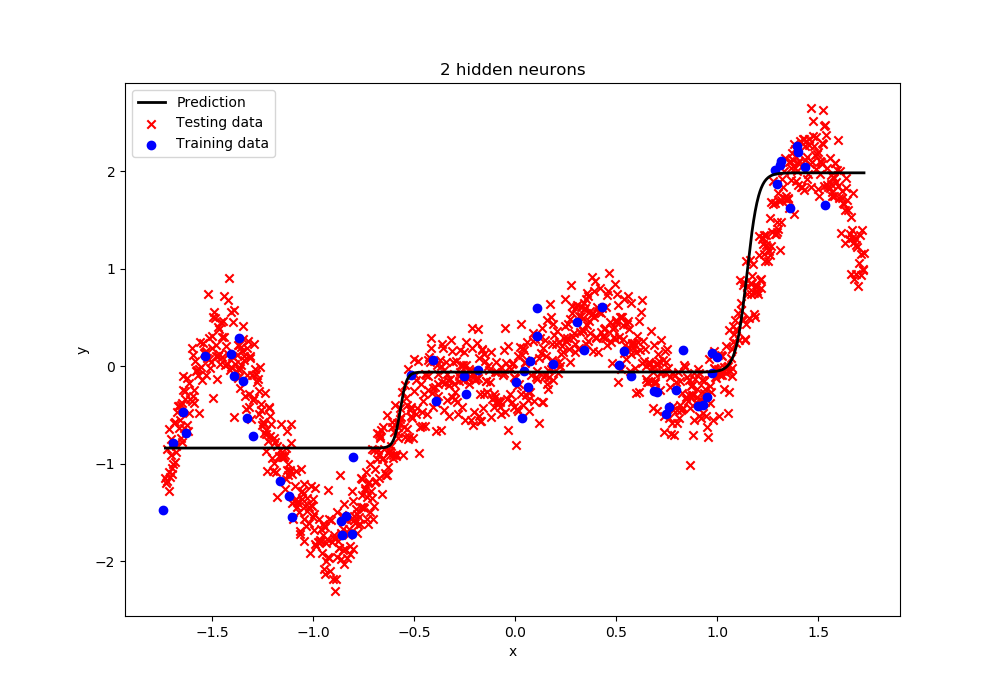
\includegraphics[width=0.5\textwidth]{ex_1_1_a_2.png}
  \caption{hidden nueron = 2}
  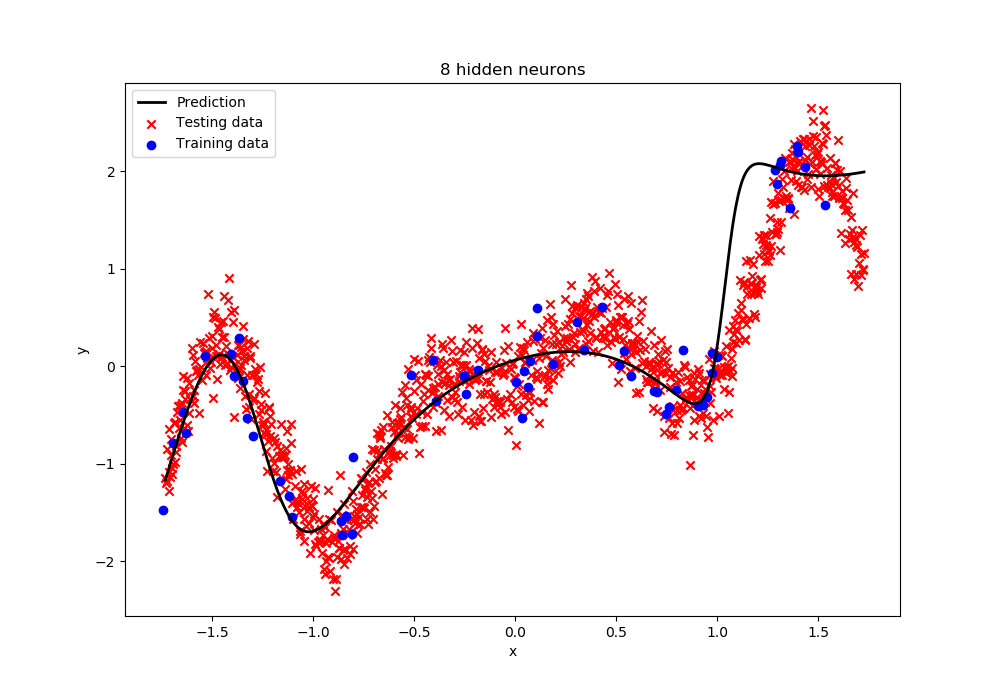
\includegraphics[width=0.5\textwidth]{ex_1_1_a_8.png}
  \caption{hidden nueron = 8}
  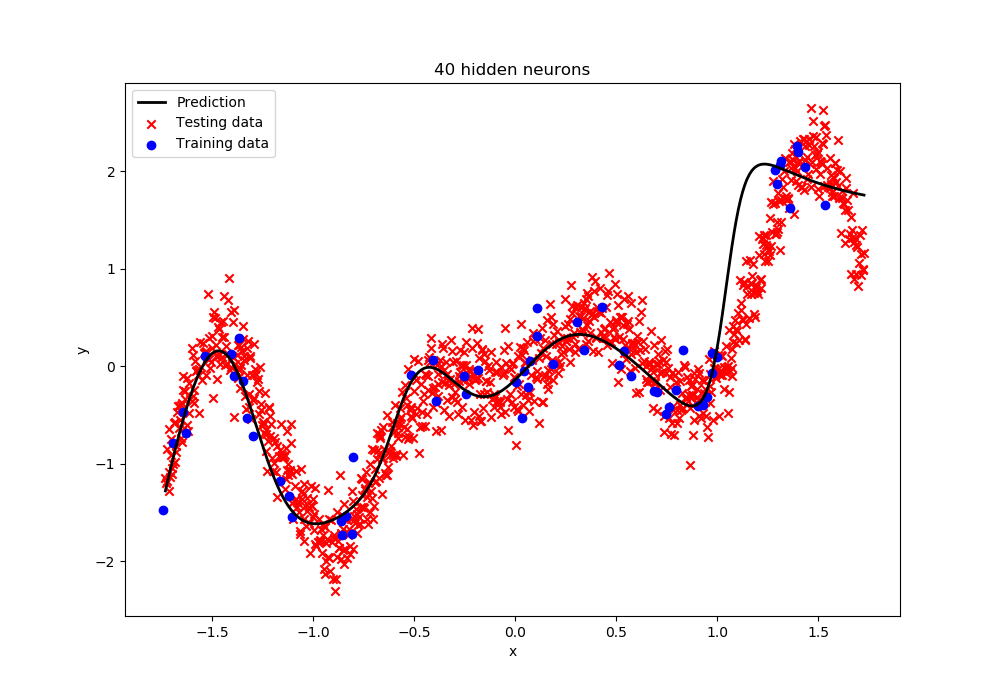
\includegraphics[width=0.5\textwidth]{ex_1_1_a_40.png}
  \caption{hidden nueron = 40}
\end{figure}

\noindent
a) 2 hidden neurons \\
It is underfitted because the dimension is too small.\\

\noindent
b) 8 hidden neurons\\
It is well fitted. \\

\noindent
c) 40 hidden neurons \\
It is the best fit to the dataset. I thought that there would be overfitting because hidden neuron number is large. However, it didn't. I think the iteration number is small like 200 so there is not enough iterations to be overfitted. Therefore, I guess if the iteration number is increased, the graph will be overfitted.\\

\subsubsection{Variability of the performance of deep neural networks}
This is  minimum, maximum, mean and standard deviation of the mean square error obtained on the training set and test set. \\
\begin{figure}[h]
  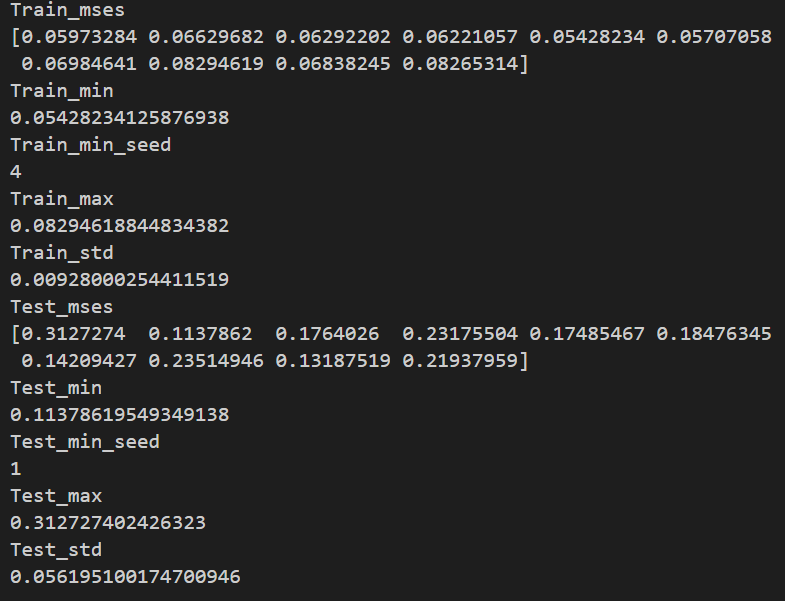
\includegraphics[width=0.5\textwidth]{ex_1_1_b.png}\\
  \caption{min, max, mean and std of MSE}
\end{figure}
Even though 5th seed is the min of train error, second seed is the min of test error. As the above result, the min of train error doesn't ensure the mind of test error. If the regression graph is overfitted to the train data, it will have really low train error but have high test error. To prevent this overfitting problem, we can use validaiton set. Before seed the train dataset to the regressor, we divide the train dataset into new train dataset and validation dataset. Therfore, we can select the seed depending not on the min of train error but on the validation error. By doing this, we can avoid overfitting problem and get more accurate regression function.\\
Even if the algorithm converged, the variability of the MSE across seeds is expected. It is because neural networks can select the graph shape freely. In the case of linear-regression and logistic regression, its dimension(graph shape) is decided by parameter. However, in the case of nerual networks, the graph shape can be decided by neural networks learning. Therefore, depending on the random seed, the optimal graph shape can be different even though the alogorithm converged. That is, the different optimal graph shape makes the variability of the MSE across seeds.\\
Standard Gardient Descent(GD) takes long time to cacluate the whole dataset gradient. Therefore, SGD is invented because of time problem. SGD doesn't calculate the whole dataset gradient but the data subset gradient. Then, it can save time. In this process, SGD will use randomness to select the data subset. Actually, it is true that the subset gradient also resembles the whole dataset gradient. Even if SGD is replaced by standard Gradient Descent, it still use randomness to initialize the neuron networks in the first step.\\
\clearpage
\subsubsection{Varying the number of hidden neurons}
This following graph is the MSE plot depending on the hidden neuron number.\\
\begin{figure}[h]
  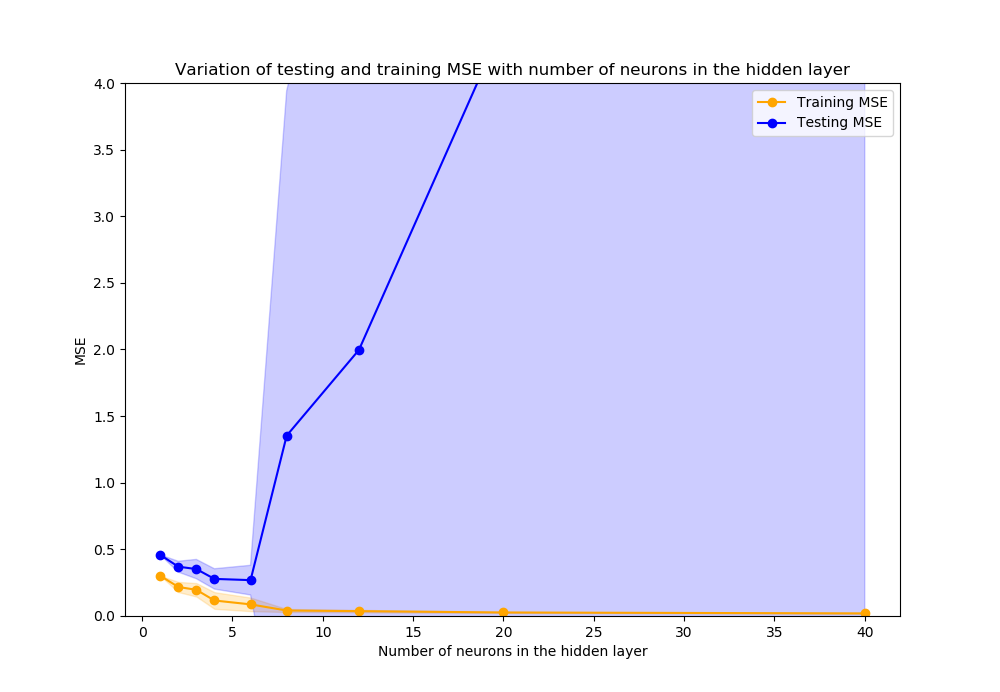
\includegraphics[width=0.5\textwidth]{ex_1_1_c.png}\\
  \caption{MSE plot with the hidden neuron number(n = [1,2,3,4,6,8,12,20,40])}
\end{figure}\\
The best value of $n_h$ independently of the choice of the random seed, is \b 6.\\
Before 6, it is underfitted Therefore, as the hidden neuron number increase, the MSE decreases.
This following graph is the learned function for one of the models trained with $n_h = 40 (max-iter=10000, tol=1e-8)$\\
\begin{figure}[h]
  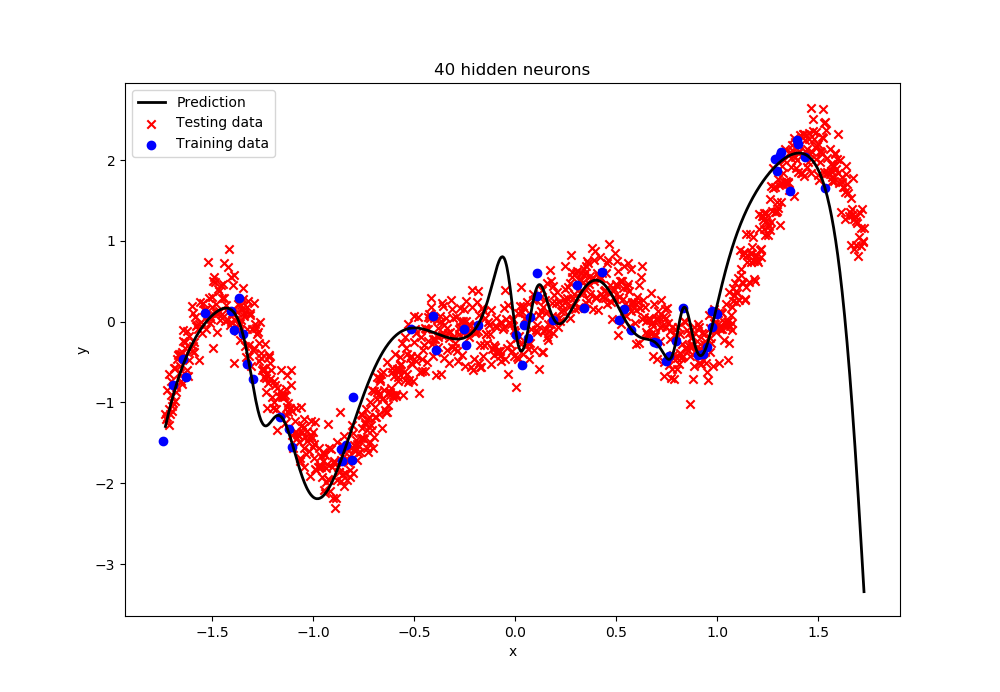
\includegraphics[width=0.5\textwidth]{ex_1_1_c_40.png}\\
  \caption{learned function of $n_h = 40 (max-iter=10000, tol=1e-8)$}
\end{figure}\\
As the figure 6 shows, the function of 40 hidden neurons is overfitted to the train dataset. And, as the figure 5 shows, the MSE of the test dataset starts increase from hidden neuron number 8 even though the MSE of train dataset still decreases. It means that it starts to be overfitted to the train dataset.\\
\clearpage
\subsubsection{Variations of MSE during training}
These plots are the the variations of the MSE with three different number of hidden neurons(2,8 and 40) for solvers('lbfgs','sgd' and 'adam')\\
\begin{figure}[h]
  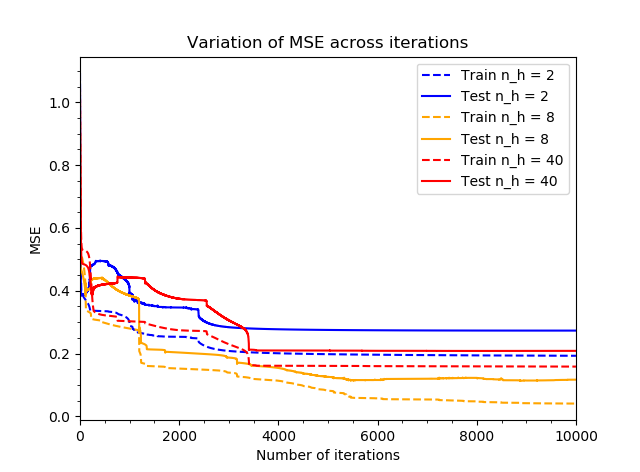
\includegraphics[width=0.4\textwidth]{ex_1_1_d_lbfgs.png}\\
  \caption{MSE plot with the hidden neuron number(2,4 and 8) and solver lbfgs}
  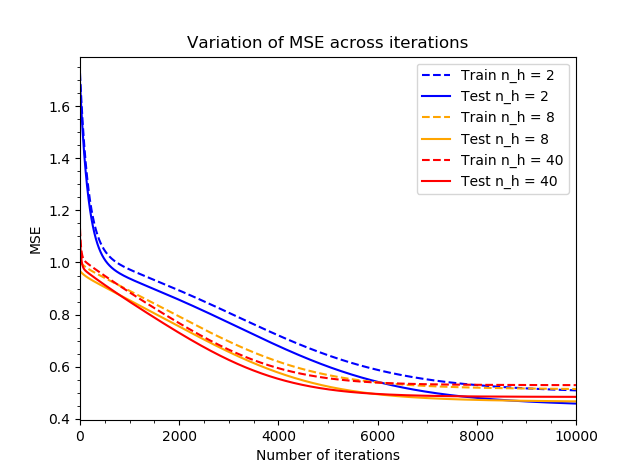
\includegraphics[width=0.4\textwidth]{ex_1_1_d_sgd.png}\\
  \caption{MSE plot with the hidden neuron number(2,4 and 8) and solver sgd}
  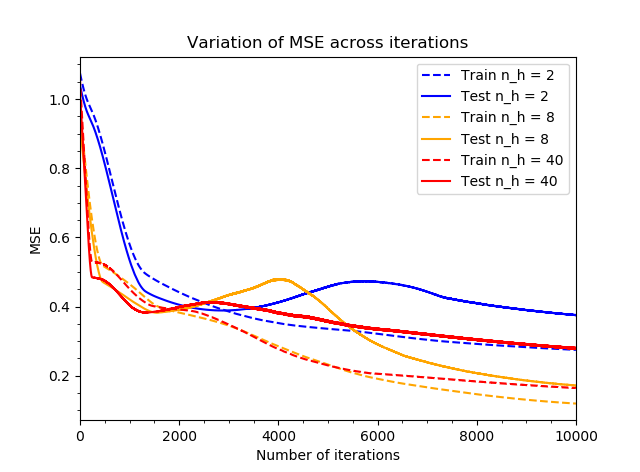
\includegraphics[width=0.4\textwidth]{ex_1_1_d_adam.png}\\
  \caption{MSE plot with the hidden neuron number(2,4 and 8) and solver adam}
\end{figure}
\\
\noindent
As Figure 7 shows, the hidden neuron number 8 has the lowest MSE. It means that the risk of overfitting increases as the number of hidden neurons increases.\\
Adam(stochastic gradient-based optimizer) seems to perform best in this problem. Actually, Adam performs well on large datasets and lbfgs(optimizer in the family of quasi-Newton methods) can converge faster and perform better on small datasets. In this problem, the size of dataset is approximately over 1000. Therfore, Adam performs best.\\
The interesting fact of Figure 9 is that it seems to overcome overfitting problem in the case of hidden neuron number 40. Adam(stochastic gradient-based optimizer) can overcome the overfitting problem by sub-sampling the whole dataset. Overfitting problem can occur because it is exactly fitted to the train set but if Adam uses sub-sampling, it can avoid this by fitting the optimal function to the data subset.\\
I think Adam works well when the number of nuerons increases. Because, when the number of neruons increases, the risk of overfitting problem also increase. Then, Adam can avoid the overfitting problem by sub-sampling. That is, Adam is more appropriate than other solvers.
\subsection{Regularized Neural Networks}
\subsubsection{Weight Decay}
The best value of $\alpha$ is $10^{-2}$. Regularization is used to overcome
overfitting. The second term in loss function makes weights are close to
zero and it makes the neural network simpler.
\begin{figure}[h]
  \begin{center}
  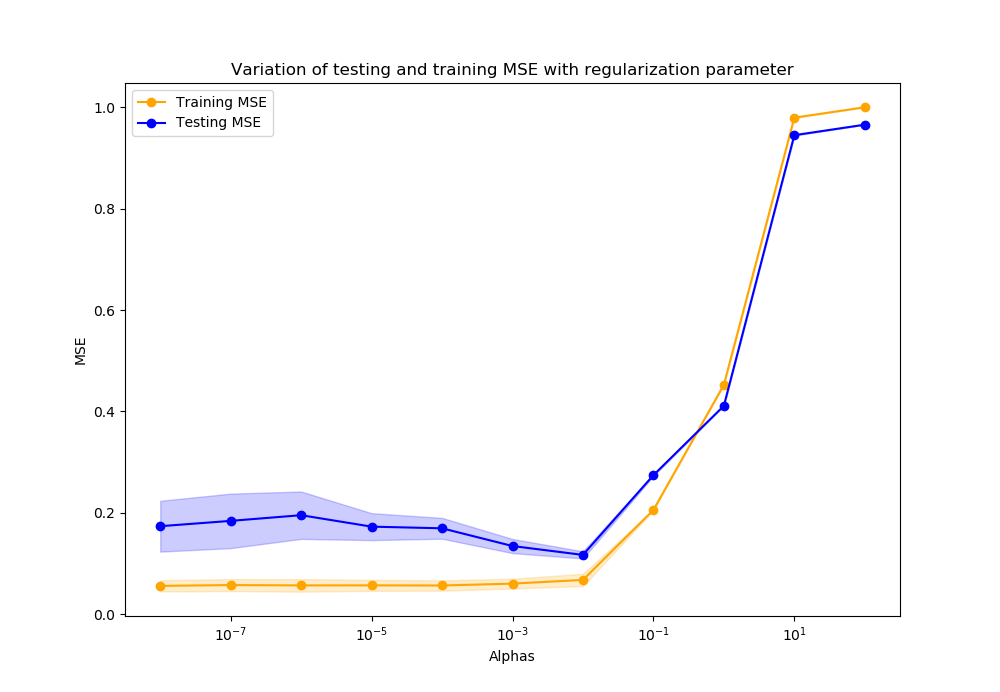
\includegraphics[width=0.8\textwidth]{ex_1_2_a.png}\\
  \caption{Plots of the variation of MSE of the training and test set with the value of $\alpha$}
  \end{center}
\end{figure}
\clearpage
\subsubsection{Early Stopping}
\begin{figure}[h]
  \begin{center}
    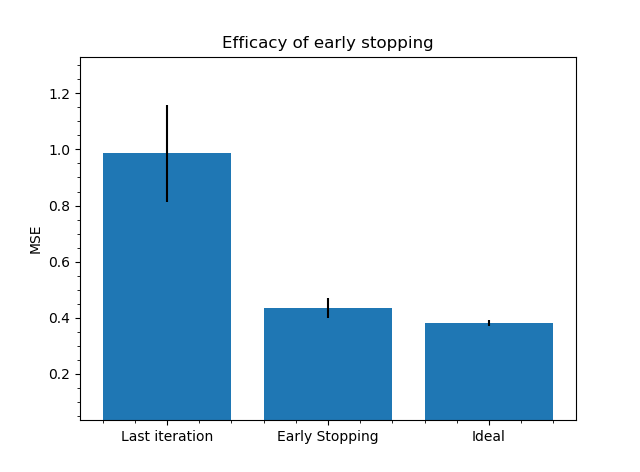
\includegraphics[width=0.5\textwidth]{ex_1_2_b.png}\\
    \caption{Early stopping MSE comparision when randint(10000)}
    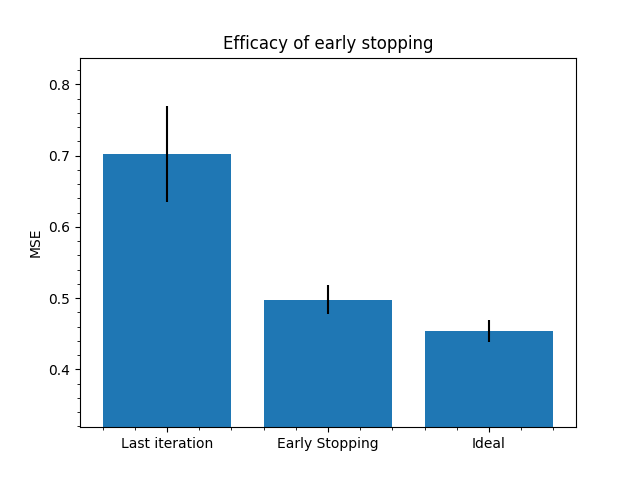
\includegraphics[width=0.5\textwidth]{ex_1_2_b_rand2.png}\\
    \caption{Early stopping MSE comparision when randint(2)}
  \end{center}
\end{figure}
As 1.1.b the variability of the MSE across seeds is expected, so it is expected that
early stopping happens at different iteration number if the random seed is differnent.
This expectation is coherent with our results. Below is a table of early stopped
iteration number and its random seed.
\begin{table}[h]
  \begin{center}
  \begin{tabular}{|
    >{\columncolor[HTML]{C0C0C0}}l |l|l|l|l|l|l|l|l|l|l|}
    \hline
    Early stopping iteration number/20 & 24 & 21 & 21 & 24 & 21 & 21 & 21 & 21 & 24 & 24 \\ \hline
    Random seed                        & 1  & 0  & 0  & 1  & 0  & 0  & 0  & 0  & 1  & 1  \\ \hline
  \end{tabular}
  \caption{np.random.randint(2)}
  \vspace{2em}
  \begin{tabular}{|
    >{\columncolor[HTML]{C0C0C0}}l |l|l|l|l|l|l|l|l|l|l|}
    \hline
    Early stopping iteration number/20 & 9    & 8    & 4    & 9    & 7    & 8    & 6    & 7    & 7    & 6    \\ \hline
    Random seed                        & 3703 & 1380 & 3277 & 3711 & 1547 & 8732 & 4389 & 6998 & 7911 & 4603 \\ \hline
  \end{tabular}
  \caption{np.random.randint(10000)}
  \end{center}
\end{table} \\
The standard form of early stopping could stop earlier than our imlementation. But it cannot ensure the minimum of MSE.
In our implementation ensures the minimum value of MSE.
\clearpage
\subsubsection{Combining the tricks}
First, to find the number of hidden neurons, settled Regularization parameter as
$10^{-2}$(because it is optimal of 1.2.a), solver as 'lbfgs'. Then, I tried to find the minimum of the mean of
testing error while changing the number of neurons from 2 to 40. When the number
of neurons was 25, the mean of testing error was minimum. After figuring out the
number of neurons, settled it as 25, I tried all three solver and 'lbfgs' was the best.
Finally, I changed regularization parameter as same range as 1.2.a.
The number of hidden neurons is 25. Regularization parameter is $10^{-3}$, Solver is 'lbfgs'.
\begin{table}[h]
  \begin{center}
    \begin{tabular}{|l|l|l|}
      \hline
      & mean                 & standard deviation    \\ \hline
      training set error   & 0.053564358953767585 & 0.0016082907699279377 \\ \hline
      validation set error & 0.06361285376287637  & 0.0022871324704669977 \\ \hline
      testing set error    & 0.1278987472019101   & 0.009530319307564717  \\ \hline
    \end{tabular}
    \caption{Mean and standard deviation of each set}
    \vspace{2em}
    \begin{tabular}{|c|c|c|}
      \hline
      Training set        & Validation set       & Testing set         \\ \hline
      0.05159202770739599 & 0.056986716577796845 & 0.11396665516400696 \\ \hline
    \end{tabular}
    \caption{Training, validation and testing error of optimal random seed}
  \end{center}
\end{table}
\clearpage
\section{Face Recognition with Neural Networks}
\subsection{Pose Recognition}
The confusion matrix is below. Pose 'left' and 'right' was seperated better than others.\\
\[
\begin{bmatrix}
  121 & 3 & 4 & 13 \\
  0 & 139 & 0 & 2 \\
  0 & 0 & 137 & 1 \\
  10 & 5 & 1 & 128
\end{bmatrix}
\]
\begin{figure}[h]
  \begin{center}
  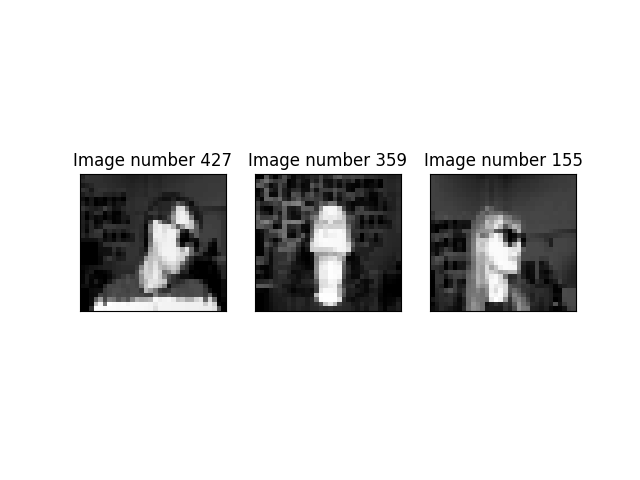
\includegraphics[width=0.5\textwidth]{ex_2_1_random.png}\\
  \caption{Random image plot}
  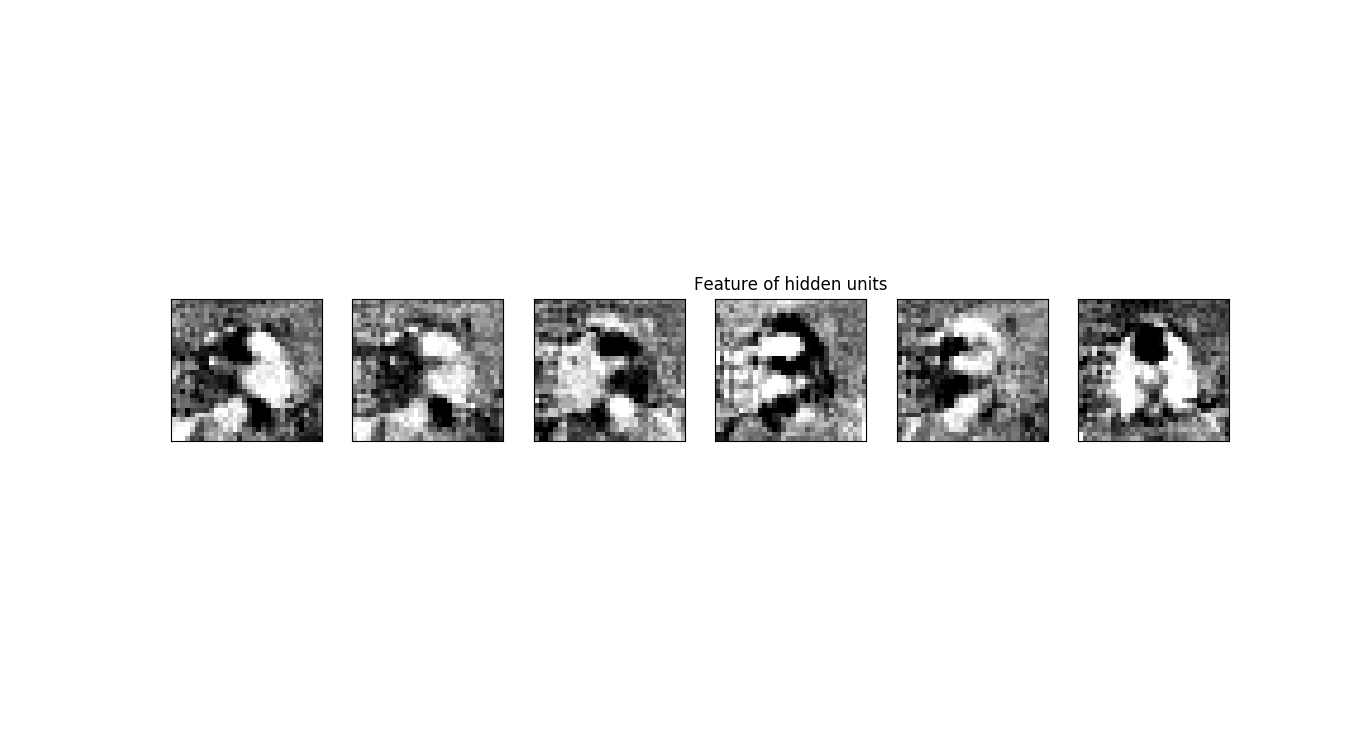
\includegraphics[width=0.7\textwidth]{ex_2_1_hidden.png}\\
  \caption{Hidden layer weights plot}
  \end{center}
\end{figure}\\
It looks like hair and sunglasses get more weights then others.
\clearpage
\subsection{Face Recognition}
\end{document}
